% !TeX spellcheck = uk_UA
\documentclass[twoside,a4paper,14pt]{vakaref-utf8}

\usepackage[T2A]{fontenc}
\usepackage[utf8]{inputenc}
\usepackage{cmap}%allows cyrillic search in pdf
\usepackage[english,russian,ukrainian]{babel}

\usepackage[intlimits]{amsmath}
\allowdisplaybreaks
\usepackage{amsthm}
\usepackage{amssymb, amsfonts}
%\usepackage[upright]{fourier} %for non-italic greek
\usepackage{enumerate,enumitem}
\usepackage{autonum}%нумерует только цитированные формулы
%\usepackage{hyperref}
\usepackage{tabularx, multirow}
\usepackage{graphicx,caption,subcaption,sidecap}
\captionsetup{labelsep=period}
\usepackage{wrapfig}
\usepackage{overpic,tikz}
\usetikzlibrary{calc}
\graphicspath{{images/}}
\usepackage{threeparttable,tablefootnote}
\usepackage{cite}

\usepackage{ulem}[normalem]
\usepackage{xcolor}
\usepackage{import}

\usepackage{geometry}
%\geometry{total={12cm,17cm},includehead}
\geometry{
	hmargin={15mm,15mm}, %20,10
	vmargin={20mm,20mm}, 
	headsep=5mm, 
	ignoreall, 
	nofoot
}

\begin{document}

%Spacing before and after equation
\setlength{\abovedisplayskip}{4pt}%
\setlength{\abovedisplayshortskip}{4pt}%
\setlength{\belowdisplayskip}{4pt}%
\setlength{\belowdisplayshortskip}{4pt}%

\author{СЕМЕНОВ АНДРІЙ КОСТЯНТИНОВИЧ}

%\authorsignature{signature-alph.png}
%\secretarysignature{signature-alph.png}

\udc{538.956; 537.9; 544.72.05; 544.77}

\title{ЕЛЕКТРОФІЗИЧНІ ВЛАСТИВОСТІ\\ БАГАТОФАЗНИХ
ДИСПЕРСНИХ СИСТЕМ}

\speciality[теоретична фізика]{01.04.02}[фізико-математичних наук]

\supervisor{Сушко Мирослав Ярославович}
  {кандидат фізико-математичних наук, доцент}
  {доцент кафедри теоретичної фізики та астрономії, 
  Одеський національний університет імені І.",І.",Мечникова}

\institution{на кафедрі теоретичної фізики та астрономії Одеського національного університету імені {І.",І.",Мечникова}}

\opponent{Лебовка Микола Іванович}
  {доктор фізико-математичних наук, професор}
  {завідувач відділу фізичної хімії дисперсних мінералів, Інститут біоколоїдної хімії імені {Ф.",Д.",Овчаренка} НАН України}

\opponent{Ледней Михайло Федорович}
  {доктор фізико-математичних наук, доцент}
  {доцент кафедри теоретичної фізики, Київський національний університет імені Тараса Шевченка}

\council{Д~41.051.04}
  [ОДЕСЬКИЙ НАЦІОНАЛЬНИЙ УНІВЕРСИТЕТ\\ імені {І.",І.",МЕЧНИКОВА}, МІНІСТЕРСТВО ОСВІТИ І НАУКИ УКРАЇНИ]
  {Одеський національний університет імені {І.",І.",Мечникова}}
  {65023 м.~Одеса, вул.~Пастера, 27, ОНУ імені {І.",І.",Мечникова},\\ Велика фізична аудиторія}
  
\secretary{Ющенко~В.",О.}{кандидат фізико-математичних наук}

\library{Одеський національний університет імені {І.",І.",Мечниковa}}
{65082 м.~Одеса, вул.~Преображенська, 24}
{http://theorphys.onu.edu.ua/thesises}

% Дата захисту і дата розсилання автореферату
% Відкрийте, коли готуєте варіант для ВАК уже після захисту
%\defencedate{2020/11/24}{14:00}
%\postdate{2020/09/23}

\maketitle

% Автореферат не має розділів, підрозділів і т. д., а лише
% структурні частини, що позначаються командою \part
\part{Загальна характеристика роботи}
\import{./}{thesis_intro-utf8}

%\newpage
\part{Основний зміст роботи}

У {\bf Вступі} обґрунтовано актуальність теми дисертації, 
визначено мету, завдання, об'єкт, предмет та методи 
дослідження. Обговорено наукову новизну і практичне
значення отриманих результатів.

В {\bf першому розділі} наведено критичний аналіз основних теорій, що використовуються для опису електрофізичних властивостей макроскопічно однорідних та ізотропних дисперсних систем і включають: класичні підходи Макс\-велла-Гарнетта та Бруггемана; 
методи знаходження меж допустимих значень ефективних параметрів;
методи вивчення задач перколяції провідності;
моделі систем частинок з морфологією тверде ядро~-~проникна оболонка, як один із способів врахування фізико-хімічних ефектів в системі;
теорія SPFT (strong-property-fluctuation theory) для сильно неоднорідних середовищ та метод компактних груп неоднорідностей (МКГ), який кладеться в основу подальших досліджень.

{\bf Другий розділ} дисертації присвячений узагальненню МКГ \cite{Sushko2007, Sushko2009, SushkoJPD2009, Sushko2017} на провідні системи з комплексною діелектричною проникністю та його застосуванню до модельної системи частинок з морфологією тверде ядро~-~проникна оболонка (див. рис.~\ref{fig:model-1layer}). 
Ця модель відома в літературі \cite{Torquato}, однак, у порівнянні з моделлю частинок тверде ядро~-~тверда оболонка, набагато менше досліджена аналітично, оскільки, по-перше, унаслідок перекривання оболонок поняття поляризовності окремої частинки стає невизначеним та, по-друге, вже для помірних товщин оболонок теорія стає суттєво багаточастинковою навіть при малих концентраціях ядер. Ми очікуємо, що за допомогою такої моделі можна краще відобразити прояви різноманітних фізико-хімічних процесів в системі, зокрема міжфазні ефекти (формування оксидних оболонок, областей з високою концентрацією дефектів, подвійних електричних шарів, областей аморфізованого полімеру тощо) та матричні ефекти (зміна властивостей самої матриці внаслідок неконтрольованого легування, забруднення, змін внутрішньої структури тощо). Ефективний аналіз моделі можливий в рамках МКГ, який дозволяє уникнути надлишкової деталізації процесів в системі.

\begin{SCfigure}[4][tb]
	\centering
	%\vspace{20pt}
	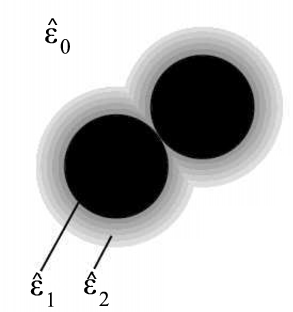
\includegraphics[width=0.25\textwidth]{particles-pen2.PNG}
	\caption{\label{fig:model-1layer}Модель макроскопічно однорідної та ізотропної тривимірної системи $\cal{D}$ частинок з морфологією тверде ядро~-~проникна оболонка, диспергованих в однорідній матриці з проникністю $\hat{\varepsilon}_0$ (біла область). Кожна частинка складається з твердого ядра радіусом $R_1$ та проникністю $\hat{\varepsilon}_1$ (чорні області) та концентричної проникної оболонки товщиною $R_2$ з радіальним розподілом проникності $\hat{\varepsilon}_2 = \hat{\varepsilon}_2(r)$ (сірі області). Всі проникності комплексні та мають структуру (\ref{eq:eps_complex}). Локальне значення проникності визначається відстанню від даної точки до центра найближчої частинки\vspace{-15pt}}
\end{SCfigure}

В {\bf підрозділі 2.1} формалізм МКГ \cite{Sushko2007, Sushko2009, SushkoJPD2009, Sushko2017} узагальнюється на провідні системи з комплексною діелектричною проникністю. Частоти зондуючого поля $\omega$ вважаються достатньо малими, щоб внесками діелектричних втрат можна було знехтувати (квазістатичне наближення). Комплексні діелектричні проникності компонентів та всієї системи моделюються у вигляді:
\begin{equation}\label{eq:eps_complex}
\hat{\varepsilon} = \varepsilon + i\,\frac{4\pi\sigma}{\omega},
\end{equation}
де $\varepsilon$, $\sigma$ -- відповідно квазістатичні дійсна частина діелектричної проникності та електрична провідність. Ефективна комплексна проникність системи $\hat{\varepsilon}_{\rm eff}$ визначається як коефіцієнт пропорційності між статистичними середніми для комплексного струму $\langle {\bf J} ({\bf r}) \rangle$ та напруженості електричного поля $\langle {\bf E}({\bf r}) \rangle$:
\begin{equation}\label{eq:eff_complex}
\langle {\bf{J}} ({\bf{r}})\rangle =
-i\frac{\omega}{4\pi}\langle \hat{\varepsilon} ({\bf{r}}) {\bf{E}}
({\bf{r}}) \rangle = -i\frac{\omega}{4\pi} \hat{\varepsilon}_{\rm
	eff} \langle {\bf{E}} ({\bf{r}}) \rangle.
\end{equation}

Знаходження $\langle {\bf{J}}\rangle$ та $\langle {\bf{E}} \rangle$ в рамках МКГ здійснюється наступним чином~\cite{Sushko2017}. Вважається, що відгук $\cal{D}$ еквівалентний відгуку допоміжної системи $\cal{S}$, утвореної диспергуванням компонентів системи $\cal{D}$ в однорідну матрицю $\cal{M}$ з поки що невідомою проникністю $\hat{\varepsilon}_{\rm f}$. Система $\cal{S}$ розглядається як сукупність макроскопічних областей (компактних груп) з лінійними розмірами $L$, набагато меншими за довжину хвилі зондуючого поля в $\cal{M}$, але достатньо великими, щоб мати властивості всієї $\cal{S}$. Локальне значення комплексної проникності в $\cal S$ записується у вигляді
$\label{eq:local_perm}
\hat{\varepsilon} ({\bf r}) = \hat{\varepsilon}_{\rm f} + \delta\hat{\varepsilon} ({\bf r}),
$
де $\delta\hat{\varepsilon} ({\bf r})$ -- внесок компактної групи в точці ${\bf r}$. Його явний вигляд залежить від розглядуваної системи. 

Середні поля і струму в рамках МКГ знаходяться таким чином \cite{Sushko2007, Sushko2009, SushkoJPD2009, Sushko2017}: розглядається рівняння поширення електромагнітного поля в $S$, записане в інтегральному представленні; за допомогою спеціального розкладу \cite{Weighofer1989} для пропагатора показується, що в квазістатичному наближенні ці середні формуються найбільш сингулярною дельта-видною частиною пропагатора. В результаті отримуємо:
\begin{equation}\label{eq:E_average}
\langle {\bf E} ({\bf r}) \rangle =  \left[ 1 + \langle \hat{Q}({\bf r}) \rangle \right] {\bf E}_0;\qquad
\langle {\bf J} ({\bf r}) \rangle = - i  \frac{\omega\hat{\varepsilon}_{\rm f}}{4\pi} \left[ 1 - 2\langle \hat{Q}({\bf r}) \rangle \right] {\bf E}_0,
\end{equation}
де 
$\label{eq:Q}
\hat{Q}({\bf r}) = \sum\limits_{s=1}^{\infty}  (-\delta\hat{\varepsilon}({\bf r})/3\hat{\varepsilon}_{\rm f})^s.
$

В {\bf підрозділі 2.2} показується, що значення $\hat{\varepsilon}_{\rm f}$ можна знайти з вимоги, щоб на межі між $\cal{M}$ та $\cal{D}$ справджувалися стандартні граничні умови для нормальних компонент комплексного струму:
$\label{eq:boundary}
\hat{\varepsilon}_{\rm f} {\bf E}_{0n} = \hat{\varepsilon}_{\rm eff} \langle {\bf E}({\bf r}) \rangle_n.
$
Разом з (\ref{eq:E_average}) вони дають $\hat{\varepsilon}_{\rm f} = \hat{\varepsilon}_{\rm eff}$. Цей результат робить теорію замкненою та разом з (\ref{eq:eff_complex})
дає рівняння для $\varepsilon_{\rm eff}$:
\begin{equation}\label{eq:general_Q}
\langle \hat{Q}({\bf r}) \rangle = 0.
\end{equation}

В {\bf підрозділі 2.3} рівняння (\ref{eq:general_Q}) застосовується для аналізу модельної дисперсної системи частинок з морфологією тверде ядро~-~проникна оболонка. $\delta\hat{\varepsilon}({\bf r})$ для цієї системи моделюється в рамках формалізму характеристичних функцій \cite{Torquato}. У випадку електрично однорідних оболонок із зовнішнім радіусом $R_2$
\begin{equation}\label{eq:delta-eps-1layer}
\delta\hat{\varepsilon} ({\bf r}) = (1 - \Pi_2 ({\bf r})) (\hat{\varepsilon}_0 - \hat{\varepsilon}_{\rm f})
+ \Pi_1 ({\bf r}) (\hat{\varepsilon}_1 - \hat{\varepsilon}_{\rm f})
+ (\Pi_2 ({\bf r}) - \Pi_1 ({\bf r})) (\hat{\varepsilon}_2 - \hat{\varepsilon}_{\rm f}),
\end{equation}
де $\Pi_1$, $\Pi_2$ -- характеристичні функції областей, зайнятих відповідно всіма ядрами (усіх чорних областей) та всіма ядрами разом з оболонками (усіх чорних та сірих областей). Підставляючи цей вираз в (\ref{eq:general_Q}), отримаємо рівняння для $\hat{\varepsilon}_{\rm eff}$:
\begin{equation}\label{eq:general_uniformshell}
	\left[1-\phi(c, \delta)\right]\frac{\hat{\varepsilon}_0
		-\hat{\varepsilon}_{\rm eff}}{2\hat{\varepsilon}_{\rm
			eff}+\hat{\varepsilon}_0} + c\,\frac{\hat{\varepsilon}_1
		-\hat{\varepsilon}_{\rm eff}}{2\hat{\varepsilon}_{\rm
			eff}+\hat{\varepsilon}_1}
	+\left[\phi(c, \delta)-c\right]\frac{\hat{\varepsilon}_2
		-\hat{\varepsilon}_{\rm eff}}{2\hat{\varepsilon}_{\rm
			eff}+\hat{\varepsilon}_2}=0,
\end{equation}
де $c = \langle \Pi_1 ({\bf r}) \rangle$ -- об'ємна концентрація ядер; $\phi(c,\delta_M) = \langle \Pi_2 ({\bf r}) \rangle$ -- об'ємна концентрація всіх ядер разом з прилеглими оболонками з відносною товщиною $\delta = (R_2 - R_1)/R_1$. Статистичні оцінки $\phi$ для рівноважної системи розглядуваних частинок відомі в літературі \cite{RikvoldP.1985}:
\begin{equation}\label{eq:phi_pen}
\begin{split}
\phi(c,&\delta) = 1 - (1-c)\exp{\left[ -\frac{(1-\psi)\phi_t}{1-c} \right]} \times \\
&\times\exp{\left[ -\frac{3c\phi_t}{2(1-c)^3} \left( 2 - 3
	\psi^{1/3} + \psi - c \left( 3\psi^{1/3} - 6\psi^{2/3} +3\psi
	\right) \right) \right]},
\end{split}
\end{equation}
де $\psi = (1+\delta)^{-3}$; $\phi_t = c/\psi$.
Цей результат дуже добре підтверджується розрахунками методами Монте-Карло \cite{Rotter2003} і використовується нами для подальших оцінок. 

Для квазістатичних провідності та діелектричної проникності за умови $|\sigma_i - \sigma_{\rm eff}| \gg \epsilon_0 \omega (\varepsilon_i + 2\varepsilon_{\rm eff})$ отримуємо рівняння:
\begin{subequations}\label{eq:general_1layer_sigma_eps}
	\begin{equation}\label{eq:general_1layer_sigma}
	(1 - \phi) \frac{\sigma_0 - \sigma_{\rm eff}}{2\sigma_{\rm eff} + \sigma_0}
	+ c \frac{\sigma_1 - \sigma_{\rm eff}}{2\sigma_{\rm eff} + \sigma_1}
	+ (\phi - c) \frac{\sigma_2 - \sigma_{\rm eff}}{2\sigma_{\rm eff} + \sigma_2} = 0,
	\end{equation}
	\begin{equation}\label{eq:general_1layer_eps}
	(1 - \phi) \frac{\varepsilon_0\sigma_{\rm eff} - \varepsilon_{\rm eff}\sigma_0}{(2\sigma_{\rm eff} + \sigma_{0})^2} 
	+ c \frac{\varepsilon_1\sigma_{\rm eff} - \varepsilon_{\rm eff}\sigma_1}{(2\sigma_{\rm eff} + \sigma_1)^2}
	+ (\phi - c) \frac{\varepsilon_2\sigma_{\rm eff} - \varepsilon_{\rm eff}\sigma_2}{(2\sigma_{\rm eff} + \sigma_2)^2} = 0.
	\end{equation}
\end{subequations}
У рамках запропонованої моделі рівняння (\ref{eq:general_1layer_sigma}) стає строгим при переході до статичної межі. 

Далі ця модель узагальнюється на випадок електрично неоднорідних оболонок.
Оболонки спершу розглядаються як сукупності великої кількості концентричних однорідних шарів, при перекриванні яких виконується правило домінування ближчих до ядра шарів над більш далекими, а потім здійснюється граничний перехід до кусково-неперервних оболонок.
Зокрема, для статичної провідності отримуємо строге співвідношення:
\begin{equation}\label{eq:general_Contlayer_sigma}
(1 - \phi) \frac{\sigma_0 - \sigma_{\rm eff}}{2\sigma_{\rm eff} + \sigma_0}
+ c \frac{\sigma_1 - \sigma_{\rm eff}}{2\sigma_{\rm eff} + \sigma_1}
+ \int\limits_0^{\delta_M} \frac{\partial \phi(c,u)}{\partial u} \frac{\sigma_2 (u) - \sigma_{\rm eff}}{2\sigma_{\rm eff} + \sigma_2 (u)} du = 0,
\end{equation}
де $\sigma_2 (u)$ -- провідність оболонки, як функція змінної 
$u = (r - R_1)/R_1$; $\delta_M$ -- відносна товщина оболонки (за її зовнішнім краєм).

Формули (\ref{eq:general_1layer_sigma_eps}) та (\ref{eq:general_Contlayer_sigma}) складають базу для подальшого аналізу в розділах 3 і 4. 


В {\bf третьому розділі} увага зосереджується на тестуванні та практичних застосуваннях рівнянь (\ref{eq:general_1layer_sigma}) та (\ref{eq:general_Contlayer_sigma}) для випадку, коли $\sigma_{0}, \sigma_1 \ll \sigma_2$, який є характерним для твердих композитних (ТКЕ) та полімерних композитних (ПКЕ) електролітів.

Тестування моделі виконується в {\bf підрозділі 3.1} шляхом порівняння її результатів з широким масивом даних числових симуляцій~\cite{Siekierski2005, Siekierski2006, Siekierski2007} для концентраційних залежностей об'ємної концентрації оболонок та статичної провідності розглядуваної модельної системи для різних діаметрів ядер та товщин оболонок двох типів: електрично однорідних~\cite{Siekierski2005, Siekierski2007}; електрично неоднорiдних з гаусовим радіальним профілем провідності~\cite{Siekierski2006}.

В рамках симуляцій~\cite{Siekierski2005, Siekierski2006, Siekierski2007} система сферично симетричних частинок із заданою товщиною оболонок замінювалася системою уявних кубічних комірок, яка потім використовувалися для побудови тривимірної ґратки резисторів. Виконаний нами аналіз показує, що якщо вимагати, щоб об'ємні концентрації твердих сферичних ядер $c$ та кубічних комірок, що їм відповідають в симуляціях, були рівними, то відносна товщина сферично симетричних оболонок $\delta$ буде меншою від відносної товщини $\delta'$, заданої в симуляціях:
\begin{equation}\label{eq:K-delta-def}
\delta = K \delta' \qquad K \leq 1.
\end{equation}
Якщо, наприклад, радіус ядра дорівнює половині довжини ребра куба, то $K=(\pi/6)^{1/3}\equiv k$; чим більша кількість комірок припадає на ядро, тим значення $K$ є ближчим до одиниці. 
В симуляціях~\cite{Siekierski2005, Siekierski2006, Siekierski2007}, довжини ребер комірок $a'$ були $0.5$~мкм, а діаметри ядер варіювалися від 3 до 11~мкм, тож відхилення $K$ від одиниці повинні бути помітними. 

В роботі  показується, що  відповідним вибором значення лише одного параметра $K$  для кожної серії симуляцій можна, по-перше, добре узгодити результати симуляцій для об'ємної концентрації з надійно перевіреним результатом (\ref{eq:phi_pen}) (див. рис.~\ref{fig:simulations-phi-a}) та, по-друге, відновити результати симуляцій для провідності за формулами (\ref{eq:phi_pen}) та (\ref{eq:general_1layer_sigma})  (рис.~\ref{fig:simulations-sigma-1layer2005-a}).
Значення $K$, використані для відтворення результатів  симуляцій для об'ємної концентрації та для ефективної провідності кожної окремої системи, незначно відрізняються, що пояснюється додатковими похибками, спричиненими більшим обсягом машинних обчислень у другому випадку.

\begin{figure*}[tb]
	\begin{subfigure}[t]{0.5\textwidth}
		\centering
		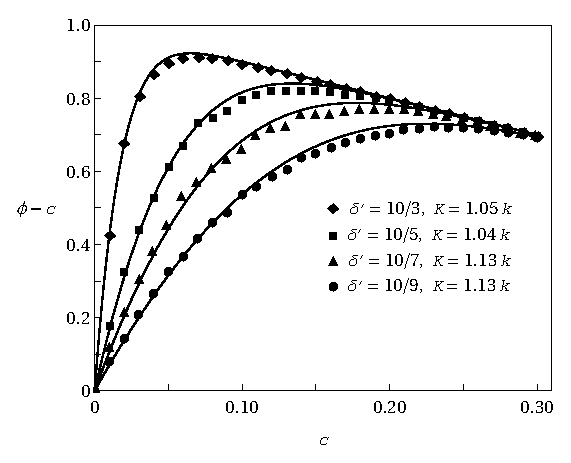
\includegraphics[height=65mm]{SiekierskiShell_107_103-9.eps}
		\caption{} \label{fig:simulations-phi-a}
	\end{subfigure}%
	~
	\begin{subfigure}[t]{0.5\textwidth}
		\centering
		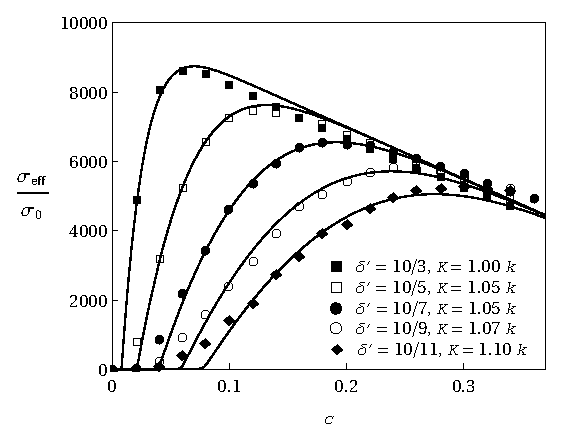
\includegraphics[height=65mm]{Fig6_Siekierski_HomogeneousLayers_t_fixed2.eps}
		\caption{} \label{fig:simulations-sigma-1layer2005-a}
	\end{subfigure}
%\vspace{-10pt}
%TODO: bigger axis text on the figs
	\caption{\label{fig:simulations-phi} 
		Залежність об'ємної концентрації оболонок $\phi-c$ (а) та ефективної провідності системи (б) від об'ємної концентрації ядер $c$ для випадку однорідних оболонок з фіксованою товщиною $t=5$~мкм та різних діаметрів ядер; $\sigma_0 {\mkern-1mu = \mkern-1mu} 1{\mkern-2mu\times\mkern-2mu} 10^{-8}$~См/см, $\sigma_1 = 1{\mkern-2mu\times\mkern-2mu} 10^{-12}$~См/см, $\sigma_2 = 1{\mkern-2mu\times\mkern-2mu} 10^{-4}$~См/см. Маркери -- дані симуляцій \cite{Siekierski2005, Siekierski2007}, суцільні лінії -- результати обробки за формулами (\ref{eq:phi_pen}), (\ref{eq:general_1layer_sigma}) та (\ref{eq:K-delta-def}) }
\vspace{-10pt}
\end{figure*}

Для відтворення даних симуляцій \cite{Siekierski2006} за допомогою формули (\ref{eq:general_Contlayer_sigma}) треба ввести ше один підгінний параметр, який враховує ефективну зміну висоти  гаусового профілю провідності сферично-симетричних оболонок при переході до системи кубічних комірок. Це дозволяє відновити всю сукупність даних симуляцій \cite{Siekierski2006} для неоднорідних оболонок.

В {\bf підрозділі 3.2} описується загальний алгоритм використання розробленої моделі для аналізу експериментальних даних, наводяться результати її застосуван\-ня до даних \cite{Liang1973} для квазістатичної провідності ТКЕ, утвореного диспергуванням частинок $\rm Al_2O_3$ в полікристалічну матрицю $\rm LiI$, та аналізується питання фізичної інтерпретації цих результатів.

Обробка експериментальних даних здійснювалася за формулами (\ref{eq:general_1layer_sigma}) і (\ref{eq:general_Contlayer_sigma}) з функціями $\sigma_2(u)$, форма яких поступово ускладнювалася від сходинки зі сталою висотою до суперпозиції сигмоїд
\begin{equation}\label{eq:GeneratingFunction3}
\frac{\sigma_2(u)}{\sigma_0} = X_{2,1} +
\frac{X_{2,2}-X_{2,1}}
{1+\exp\left[-\frac{u-\Delta_1}{\alpha}\right]}
+\frac{X_{2,3}-X_{2,2}}{1+\exp\left[-\frac{u-\Delta_2}{\alpha}\right]}
+\frac{1-X_{2,3}}{1+\exp\left[-\frac{u-\Delta_3}{\alpha}\right]},
\end{equation}
поки не досягалося достатнього узгодження теорії з експериментом. Тут величини $X_{2,m}$, $\Delta_m$ ($m=1,2,3$), $\alpha$ та, в загальному випадку, відносна провідність ядра $x_1=\sigma_1/\sigma_0$ -- підгінні параметри. При $\alpha \to 0$ (\ref{eq:GeneratingFunction3}) має вигляд трьох сходинок, що відповідає моделі тришарових оболонок, при цьому $X_{2,m}$ та $\Delta_m$ набувають змісту відносних провідностей шарів $x_{2,m} = \sigma_{2,m}/\sigma_0$ та  відносного положення їх країв $\delta_m = (R_{2,m}-R_1)/R_1$.

\begin{figure}[tb]
	\centering
	\begin{subfigure}[c]{0.45\textwidth}
		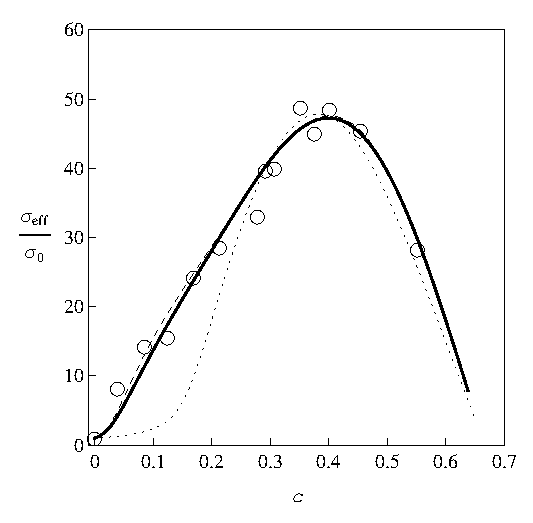
\includegraphics[width=\textwidth]{Fig12_Liang_LiI-Al2O3-Processing.eps}
		\caption{} \label{fig:Liang_LiI-Al2O3-Processing-a}
	\end{subfigure}%
	\quad
	\begin{subfigure}[c]{0.35\textwidth}
		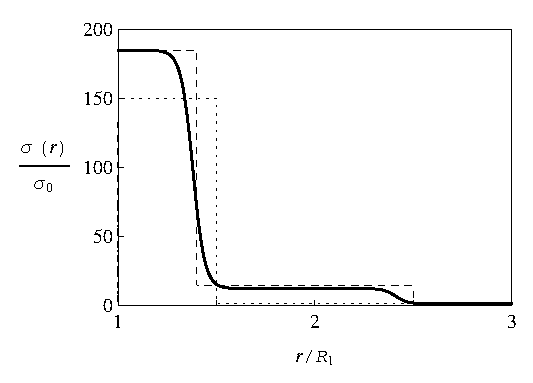
\includegraphics[width=\textwidth]{Fig13_Liang_LiI-Al2O3-Profile.eps}\\ 
		%TODO: bigger. and maybe the lower fig on top?
		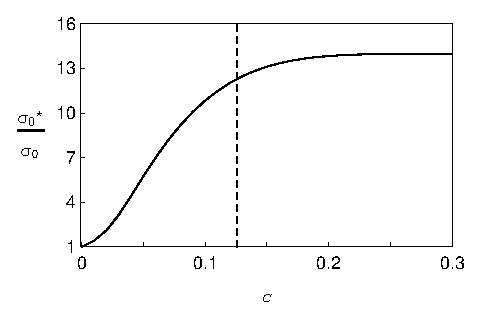
\includegraphics[width=\textwidth]{Liang-matrix-a06.eps}
		\caption{} \label{fig:Liang_LiI-Al2O3-Processing-b}
	\end{subfigure}%
%\vspace{-10pt}
	\caption{\label{fig:Liang_LiI-Al2O3-Processing} (а) Залежність $\sigma_{\rm eff}$ ТКЕ $\rm{LiI-Al_2O_3}$ від концентрації частинок $\rm Al_2O_3$: $\circ$ -- експериментальні дані \cite{Liang1973}; лінії -- результати їх обробки за (\ref{eq:general_Contlayer_sigma}) з профілями провідності оболонки (б, зверху); (б, знизу) -- залежність провідності матриці
		від $c$ (штрихована лінія -- поріг перколяції $c_{c} \approx 0.126$ в системі зовнішніх шарів)}
\vspace{-10pt}
\end{figure}

Аналіз показує, що вже модель двошарової оболонки з параметрами шарів $x_{2,1} =185$,  $\delta_1=0.40$ та $x_{2,2} =14$,  $\delta_2= 1.40$ є достатньою для опису даних \cite{Liang1973} (див рис. \ref{fig:Liang_LiI-Al2O3-Processing}). ``Розмивання'' профілю $\sigma_2(u)$ шляхом збільшення значення $\alpha$ від 0 до 0.03 (при незначній зміні решти параметрів) практично не поліпшує результати. Для цієї моделі рівняння (14) еквівалентне системі двох рівнянь
\begin{subequations}
\begin{equation}\label{eq:conductivityNewMatrix}
\left[1-\phi(c, \delta_1)\right]\frac{\sigma_0^* -\sigma_{\rm
		eff}}{2\sigma_{\rm eff}+\sigma_0^*} + c\,\frac{\sigma_1
	-\sigma_{\rm
		eff}}{2\sigma_{\rm eff}+\sigma_1} 
+\left[\phi(c, \delta_1)-c\right]\frac{\sigma_{2,1} -\sigma_{\rm
		eff}}{2\sigma_{\rm eff}+\sigma_{2,1}}=0,
\end{equation}
\begin{equation}\label{eq:sigma0-vs-c}
\begin{split}
(1 - \phi(c,\delta_1))\frac{\sigma_0^* - \sigma_{\rm
		eff}}{2\sigma_{\rm eff} + \sigma_0^*}= &(1 - \phi(c,\delta_2))
\frac{\sigma_0 - \sigma_{\rm eff}}{2\sigma_{\rm eff} + \sigma_0} +\\
&+ (\phi(c,\delta_2) - \phi(c,\delta_1)) \frac{\sigma_{2,2} -
	\sigma_{\rm eff}}{2\sigma_{\rm eff} + \sigma_{2,2}}.
\end{split}
\end{equation}
\end{subequations}
Рівняння (\ref{eq:conductivityNewMatrix}) описує ефективну провідність системи, утворену диспергуванням  твердих частинок, оточених приповерхневими проникними шарами з товщиною $\delta_1$ та провідністю $x_{2,1}$, в матрицю, провідність якої $\sigma^*_0$ змінюється з концентрацію ядер згідно з рівнянням (\ref{eq:sigma0-vs-c}) (нижній рис.~\ref{fig:Liang_LiI-Al2O3-Processing-b}).

На основі цього робиться висновок, що  параметри модельного профілю $\sigma_2(u)$, отримуваного з обробки експериментальних даних за допомогою моделі дисперсної системи як сукупності частинок типу тверде ядро~-~проникна оболонка, ефективно описують вплив різних фізичних механізмів на формування ефективної провідності системи. Наявність кількох добре виражених ділянок на цьому профілі вказує на зміну відносної ролі цих механізмів зі зміною концентрації диспергованих частинок -- із зростанням концентрації ядер домінуюча роль переходить до більш внутрішніх шарів.
Зокрема, для системи $\rm LiI-Al_2O_3$ зовнішня ділянка профілю $\sigma_2(u)$ враховує внесок матричних процесів у формуванні $\sigma_{\rm eff}$. Ними можуть бути неконтрольоване легування матриці при підготовці експериментальних зразків, накопичення дислокацій та формування високопровідних шляхів для транспорту іонів тощо \cite{Dudney1989}. 
Ближня ділянка вказує на існування високопровідного шару (товщиною приблизно $2$~мкм), наприклад, просторового заряду навколо частинок $\rm Al_2O_3$, спричиненого накопиченням точкових дефектів \cite{Maier1985}. Отримані нами оцінки добре узгоджуються з результатами $\delta_1=0.4$ та $x_{2,1}=324$ \cite{Jiang1995b} для кубічної ґратки з ідеальним рівноважним розподілом кубічних частинок, отриманими поєднанням перколяційної теорії та моделі шару просторового заряду.

В {\bf підрозділі 3.3} наводяться результати застосування аналогічної процедури до опису експериментальних даних~\cite{Przl1995, Wiec1994} з концентраційних залежностей електричної провідності полімерних композитних електролітів на основі поліетилен-оксиду (PEO) та PEO з приєднаним оксіметиленом (OMPEO) з додаванням солей $\rm NaI$ або $\rm LiClO_4$. В якості наповнювачів виступали провідні ($\rm Na_{3.2}Zr_2P_{0.8}Si_{2.2}O_{12}$ (NASICON)) чи непровідні ($\rm \theta- Al_2O_3$) частинки, або полімер іншого сорту (поліакриламід (PAAM)), що не змішувався з полімером матриці. Результати (див. рис.~\ref{fig:PEO-NaI}) показують наявність двох-трьох чітко виражених ділянок на отриманих профілях провідності.

\begin{figure*}[bt]
	\centering
	\begin{subfigure}[c]{0.45\textwidth}
		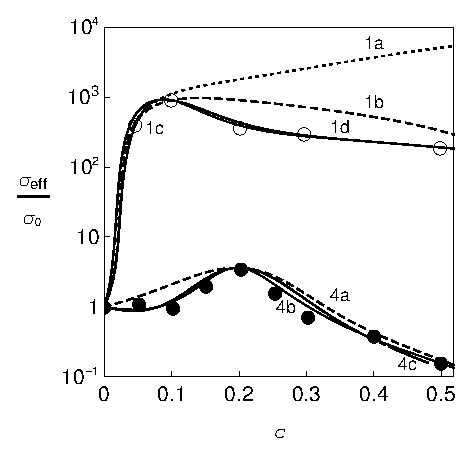
\includegraphics[width=\textwidth]{Fig3_PEO-NASICON_NaI_OMPEO-PAAM_LiClO4.eps}
		\caption{} \label{fig:OMPEO-LiClO4-a}
	\end{subfigure}%
	~
	\begin{subfigure}[c]{0.38\textwidth}
		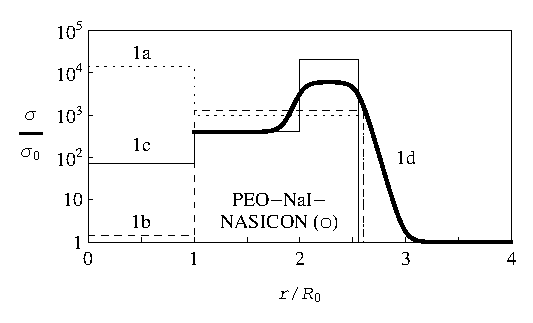
\includegraphics[width=\textwidth]{Fig2_PEO-NaI_NASICON_Profile.eps}
		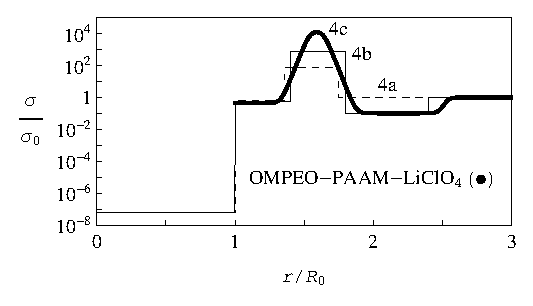
\includegraphics[width=\textwidth]{Fig3_OMPEO-PAAM_LiClO4_Profile.eps}
		\caption{} \label{fig:OMPEO-LiClO4-b}
	\end{subfigure}
%\vspace{-10pt}
	\caption{\label{fig:PEO-NaI} 
		(а) Залежності ефективних провідностей ПКЕ PEO--NaI--NASICON \cite{Przl1995} ($\circ$) та OMPEO--LiClO$_4$--PAAM (з молярною концентрацією LiClO$_4$ 10~\%, після відпалу)
		\cite{Wiec1994} ($\bullet$) від $c$ та результати їх обробки за (\ref{eq:general_Contlayer_sigma}) для модельних одночастинкових профілів провідності (б)}
\vspace{-10pt}
\end{figure*}

Центральна ділянка $\sigma_2(u)$ (рис.~\ref{fig:OMPEO-LiClO4-b}) характеризується провідністю, що на кілька порядків перевищує провідність матриці. Цей результат узгоджується з експериментально перевіреним фактом \cite{nanocomp2008} про формування навколо частинок в ПКЕ аморфізованих областей з відносно високою провідністю, яка є результатом підвищеної сегментарної гнучкості полімерних ланцюгів та, відповідно, підвищеної рухливості іонів розчиненої солі в цих областях. 

Найближча до ядер  ділянка $\sigma_2(u)$ описує сумарний ефект кількох можливих процесів: затруднення, під впливом твердих частинок, руху сегментів полімерних ланцюгів  в безпосередньому їх околі (так званий ``stiffening effect'' -- ефект затвердіння \cite{Wiec1994}), що веде до зниження локальної провідності; залежність цього значення від провідних властивостей частинок, а отже і природи міжфазної поверхні; нерегулярність форми частинок. Крім того, отримуване на основі наших обробок значення провідності $\sigma_1\approx 0.690$~мкСм/см для частинок NASICON в ПКЕ суттєво відрізняється від провідності $\sigma_1\approx 138$~мкСм/см до їх диспергування в ПКЕ. Цей результат (рис.~\ref{fig:OMPEO-LiClO4-a}, лiнiї 1) вказує на формування на поверхні частинок тонкої слабкопровiдної оболонки \cite{Ploch1988}. 

Найвіддаленіша ділянка $\sigma_2(u)$ ефективно відображає залежність провідності матриці від $c$. Зокрема, з наших результатів випливає, шо провідність  матриці в  ПКЕ $\rm OMPEO-LiClO_4-PAAM$ знижується в порівнянні з провідністю чистого аморфного OMPEO. Це пояснюється зв'язуванням іонами солі поодиноких молекул PAAM, розподілених в матриці поза межами практично непровідних глобул PAAM \cite{Wiec1994}.
%іонів солі окремими ланцюжками PAAM, що залишилися поза межами практично  непровідних глобул PAAM \cite{Wiec1994}.

\begin{figure*}[tb]
	\centering
	\begin{subfigure}[t]{0.45\textwidth}
		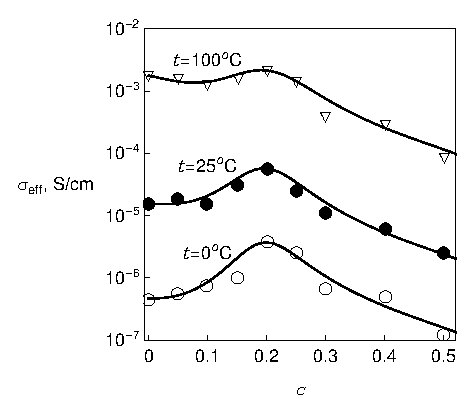
\includegraphics[width=\textwidth]{Fig6_Isochores2.eps}
		\caption{} 
		\label{fig:OMPEO-LiClO4-Temp-a}
	\end{subfigure}%
	\quad
	\begin{subfigure}[t]{0.47\textwidth}
		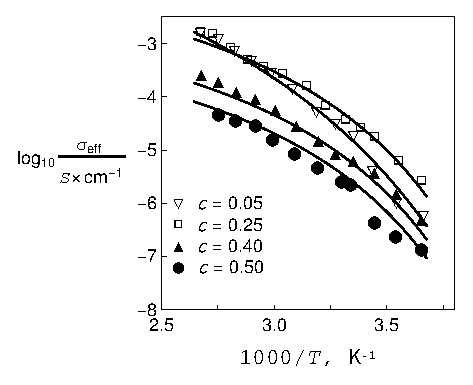
\includegraphics[width=\textwidth]{Fig8_TemperatureDependence_4.eps}
		\caption{} \label{fig:OMPEO-LiClO4-TempDependence}
	\end{subfigure}%
	%\vspace{-10pt}
	\caption{\label{fig:OMPEO-LiClO4-Temp} Залежності $\sigma_{\rm eff}$ ПКЕ OMPEO--LiClO$_4$--PAAM \cite{Wiec1994} від (а) об'ємної концентрації PAAM при фіксованих температурах та (б) температури при фіксованих значеннях концентрації PAAM.
		Неперервні лінії: результати розрахунків за (\ref{eq:general_Contlayer_sigma}) з використанням закону VTF для шарів та матриці
		в рамках тришарової моделі}
	\vspace{-10pt}
\end{figure*}

У силу різної фізичної природи задіяних механізмів параметри різних ділянок $\sigma_2(u)$ повинні по-різному залежати від температури. Це припущення використовується нами для подальшого тестування та розширення теорії та досліджується на прикладі температурної залежності $\sigma_{\rm eff}$ ПКЕ $\rm OMPEO-LiClO_4-PAAM$ \cite{Wiec1994}. 
Оскільки три ділянки профілю $\sigma_2(u)$  формуються процесами в  областях з різним ступенем аморфності, температурна залежність параметрів $x_{2,m}$ моделюється за допомогою трипараметричного емпіричного закону Фогеля~-~Таммана~-~Фульхера (VTF).
Відповідні параметри VTF для цих ділянок та матриці знаходяться шляхом обробки трьох ізотерм $\sigma_{\rm eff} (c,T)$ в рамках тришарової моделі (рис.~\ref{fig:OMPEO-LiClO4-Temp-a}) при фіксованих значеннях інших параметрів моделі. 
Отриманих значень виявляється достатньо, щоб відновити температурні залежності $\sigma_{\rm eff}$ зразків композиту з різними значеннями концентрації PAAM в усьому дослідженому температурному інтервалі (рис.~\ref{fig:OMPEO-LiClO4-TempDependence}). 

У {\bf четвертому розділі} аналізуються властивості розв'язків рівнянь (\ref{eq:general_1layer_sigma_eps}) та (\ref{eq:general_Contlayer_sigma}) для випадку $\sigma_0 \ll \sigma_2 \lesssim \sigma_1$ та профілю провідності оболонок в (\ref{eq:general_Contlayer_sigma}) виду
\begin{equation}\label{eq:profile-perc}
\sigma_2 (u) = \sigma_{\rm max} \exp [-(u/\delta)^p \ln(\sigma_{\rm max}/\sigma_{\rm min})],
\end{equation}
при різних значеннях степеня $p\geq 1$ ($\sigma_{\rm max}$ та $\sigma_{\rm min}$ -- значення провідності оболонки при $u=0$
та $u=\delta$, відповідно) та розглядаються результати застосування цих розв'язків до опису явища електричної перколяції в реальних системах типу провідник~-~ізолятор з міжфазним шаром.

В {\bf підрозділах 4.1 та 4.2} показується, що для вказаних значень провідностей ком\-понентів поведінка $\sigma_{\rm eff}$ та $\varepsilon_{\rm eff}$ має перколяційний характер. Поріг перколяції $c_c$, який відповідає утворенню перколяційного кластера в системі проникних оболонок із заданою $\delta$, визначається як значення концентрації, при якому з'являється нетривіальний розв'язок рівняння (\ref{eq:general_1layer_sigma}) для системи з непровідною матрицею ($\sigma_0 = 0$):
\begin{equation}\label{eq:threshold}
\phi(c_c, \delta) = 1/3.
\end{equation}

Поведінку ефективної провідності в околі $c_c$ можна подати у вигляді $\sigma_{\rm eff}\sim (c_c - c)^{-s_{\rm eff}}$ при $c < c_c$ та $\sigma_{\rm eff}\sim(c - c_c)^{t_{\rm eff}}$ при $c > c_c$, при цьому показники $s_{\rm eff}$ та $t_{\rm eff}$ для розвинутої моделі не є універсальними, а залежать від значень відносної провідності матриці $x_0 = \sigma_0/\sigma_1$ та концентраційного інтервалу $[c_1,c_2]$, на якому вони визначаються (див. рис.~\ref{fig:teff-seff}). Зазначимо, що індекс $t_{\rm eff}$ визначається для матриці з нульовою провідністю, тому при його оцінці до профілю (\ref{eq:profile-perc}) додавалась величина $(-\sigma_{\rm min})$, щоб виконувалась рівність $\sigma_2(\delta) = 0$.
Для аналогічних двовимірних моделей неуніверсальність степеневих показників підтверджується симуляціями \cite{Myroshnychenko2008}. Такі залежності індексів $s_{\rm eff}$ та $t_{\rm eff}$ дозволяють пояснити широкий спектр їх експериментальних значень ($s_{\rm eff} \approx 0.7 \div 1.0$; $t_{\rm eff} \approx 1.5 \div 4$).

Перколяційний перехід в системі ядер в рамках моделі відбувається при фіксованій концентрації $c_c = 1/3$. За умови $\sigma_2 \ll \sigma_1$ провідність демонструє ``подвійну перколяцію''. Схожий ефект спостерігається, наприклад, в системах утворених диспергуванням нанотрубок в рідко-кристалічну матрицю \cite{Tomylko2015}. 

Діелектрична проникність в околі вказаних порогів перколяції має максимум.


\begin{figure}[htb]
	\centering
	\begin{subfigure}[c]{0.45\textwidth}
		\begin{overpic}[width=\textwidth]{teff3-thick.eps}
			\put(25,55){\footnotesize $\sigma_0=0$}
		\end{overpic}
		\caption{$\sigma_{\rm min} = 10^{-10}\sigma_1$} 
		\label{fig:teff-seff-a}
	\end{subfigure}%
	\quad
	\begin{subfigure}[c]{0.45\textwidth}
		\begin{overpic}[width=\textwidth]{seff3-thick.eps}
			\put(20,25){\footnotesize $c_1 = 0.24$}
			\put(20,18){\footnotesize $c_2 = 0.25$}
		\end{overpic}
		\caption{$\sigma_{\rm min} = 5\times 10^{-5}\sigma_1$} \label{fig:teff-seff-b}
	\end{subfigure}%
	%\vspace{-10pt}
	\caption{\label{fig:teff-seff}
		Залежності ефективних критичних індексів: (а) $t_{\rm eff}$ від $c_2$
		при фіксованому $c_1$ та непровідній матриці; (б)
		$s_{\rm eff}$ від $x_0 = \sigma_0/\sigma_1$ з фіксованими $c_1$ та $c_2$. Штрих-пунктирні лінії -- дані для електрично однорідного профілю при $\sigma_2/\sigma_1 = 5 \times 10^{-5}$; неперервні та штриховані лінії -- результати для профілю (\ref{eq:profile-perc}) при, відповідно, $p=1$ та $p=2$, $\sigma_{\rm max} = \sigma_1$. Вертикальні точкові лінії відповідають значенням $c_1$; $\delta = 0.1$ ($c_c \approx 0.251$)}
	\vspace{7pt}
\end{figure}

\begin{figure}[!h]
	\centering
	\begin{subfigure}[c]{0.45\textwidth}
		\begin{overpic}[height=60mm]{chen-grannan-eps.eps}
			\put(19,90){\footnotesize $\circ$ -- $\varepsilon_0 = 5.0$, $\delta = 0.194$,}
			\put(29,83){\footnotesize $s_{\rm eff} = 0.72$}
			\put(17,70){\footnotesize $\triangle$ -- $\varepsilon_0 = 7.0$, $\delta = 0.150$,}
			\put(29,63){\footnotesize $s_{\rm eff} = 0.74$}
		\end{overpic}
		\caption{} 
		\label{fig:KCl-Ag-a}
	\end{subfigure}%
	\quad
	\begin{subfigure}[c]{0.45\textwidth}
		\begin{overpic}[height=60mm]{chen-grannan-s2.eps}
			\put(65,30){\footnotesize $\delta \approx 0.162$}
		\end{overpic}
		\caption{} \label{fig:KCl-Ag-b}
	\end{subfigure}%
	\caption{\label{fig:KCl-Ag} Залежності (а) $\varepsilon_{\rm eff}$ та (б) $\sigma_{\rm eff}$ нанокомпозитів $\rm KCl-Ag$ від концентрації частинок $\rm Ag$ за експериментальними даними \cite{Grannan1981, ChenI.-G.1986}. Неперервні лінії на (а) та штрих-пунктирні на (б) -- обробки, отримані за (\ref{eq:general_1layer_sigma_eps}) при $\sigma_0 \approx 3.13 \times 10^{-8}$~См/м, $\sigma_1 \approx 6.25 \times 10^7 $~См/м, $\sigma_2 \approx 250$~См/м; неперервні лінії на (б) -- обробки за (\ref{eq:general_Contlayer_sigma}) та (\ref{eq:profile-perc}) при $p=3.2$, $\sigma_{\rm max} = \sigma_1$, $\sigma_{\rm min}=1$~См/м, $\sigma_0 \approx 4.69\times 10^{-8}$~См/м, $\sigma_1 \approx 6.25 \times 10^7 $~См/м; точкові лінії -- скейлінгові підгонки, запропоновані в \cite{Grannan1981} для даних при $c > 0.11$}
	\vspace{-10pt}
\end{figure}

В {\bf підрозділі 4.3} показується (рис. \ref{fig:KCl-Ag-a}, \ref{fig:KCl-Ag-b}), що вже модель однорідної оболонки ($p=0$, $\sigma_2 = \sigma_{\rm min}$) при $c < c_{\rm c}$ достатньо добре описує експериментальні дані \cite{Grannan1981} для діелектричної проникності та \cite{ChenI.-G.1986} для електричної провідності спеціально підготовленої системи на основі KCl з наночастинками Ag з середнім радіусом $R\approx 10$~нм, покритими проникним оксидним шаром. 
Зокрема, формула (\ref{eq:general_1layer_eps}) описує експериментальні дані краще за скейлінгові закони (див. рис.~\ref{fig:KCl-Ag-a}). 
При  $c > c_{\rm c}$ перекривання оболонок суттєві, а тому важливою стає їх внутрішня структура, тож для відновлення даних з провідності (рис. \ref{fig:KCl-Ag-b}) використано рівняння (\ref{eq:general_Contlayer_sigma}) з профілем (\ref{eq:profile-perc}).
Отримані оцінки для $\delta \approx 0.14 \div 0.18$ близькі до прогнозованих експериментаторами $\delta \approx 0.1$.
Неоднорідна структура профілю оксидної оболонки може бути результатом механізму тунелювання електронів, що підтверджується його формою та оцінками характерної довжини тунелювання ($0.4\div 1$~нм) \cite{Ambrosetti2009}. 
Внески в профіль ефектів, які відіграють роль при високих концентраціях (наприклад, spill-out ефекту) було неможливо виявити внаслідок відсутності експериментальних даних для цих концентрацій.


В {\bf п'ятому розділі} МКГ застосовується для критичного аналізу диференціальних схем обчислення ефективної діелектричної проникності (електричної провідності) невпорядкованих систем та на прикладі системи твердих діелектричних куль в діелектричній матриці демонструється їх  обмеженість. Для цього в {\bf підрозділі~5.1} рівняння (\ref{eq:general_Q}) у вигляді $$\left\langle \delta\varepsilon({\bf r})(3\varepsilon_{\rm eff} + \delta\varepsilon({\bf r}))^{-1} \right\rangle = 0$$
%\begin{equation}\label{eq:general_Q_diff0}
%	\left\langle \frac{\delta\varepsilon({\bf r})}{3\varepsilon_{\rm eff} + \delta\varepsilon({\bf r})} \right\rangle = 0
%\end{equation}
використовується для побудови диференціальних рівнянь для ефективної проникності. Якщо при додаванні до системи інфінітезимальної порції частинок з об'ємною концентрацією $\Delta c$ її ефективна діелектрична проникність стає $\varepsilon_{\rm eff} + \Delta\varepsilon$, то проникність компактної групи в точці $\bf r$ з урахуванням поправок того ж порядку малості за $\Delta c$ та $\Delta\varepsilon$ дається трьома доданками
\begin{equation}\label{eq:delta-Brug-diff}
\begin{split}
\widetilde{\delta\varepsilon} ({\bf r}) \approx \delta\varepsilon ({\bf r})+ \delta\varepsilon_{\rm ABM}^{(l)} ({\bf r}) + \delta\varepsilon_{\rm ABM}^{(h)} ({\bf r}) ,
\end{split}
\end{equation}
де $\delta\varepsilon$ -- внесок в локальну проникність заданої компактної групи до додавання частинок, а внески $\delta\varepsilon_{\rm ABM}^{(l)}$, $\delta\varepsilon_{\rm ABM}^{(h)}$ враховують  вплив на проникність цієї компактної групи відповідно нових частинок та зміни матриці внаслідок їх додавання. 
Присутність $\delta\varepsilon$ в (\ref{eq:delta-Brug-diff}) означає, що ефективна проникність новоутвореної системи залежить не лише від доданого компоненту, але й від властивостей системи на момент його додавання. Але ця обставина фактично ігнорується при застосуванні диференцальних схем. Зокрема, відому асиметричну модель Бруггемана (АМБ) дістаємо у результаті інтегрування диференціального рівняння, яке отримуємо, знехтувавши внесками $\delta\varepsilon $ та $\delta\varepsilon_{\rm ABM}^{(h)}$ 
(або $\delta\varepsilon $ та $\delta\varepsilon_{\rm ABM}^{(l)}$), що можливо лише за наступних умов: 
а) концентрація компоненту, що додається, є малою;
б) різниці між діелектричними проникностями компонентів малі.
Якщо ж виконується тільки перша умова, що відповідає АМБ, то лише внесок $\delta\varepsilon_{\rm ABM}^{(h)}$ ($\delta\varepsilon_{\rm ABM}^{(l)}$) є другого порядку малості. Нехтуючи цим внеском та інтегруючи отримане диференціальне рівняння, ми отримаємо модифіковану АМБ. 

В {\bf підрозділі~5.2} показується, що отримані нові співвідношення не задовольняють межі Хашина-Штрікмана, що свідчить про їх обмеженість та неможливість  екстраполяції розв'язків диференціальних рівнянь, побудованих для вузьких концентраційних інтервалів, на весь концентраційний інтервал. Формули АМБ задовольняють ці межі, але вони застосовні лише до дуже вузького класу систем, що визначається зазначеними умовами а) та б).


\part{Висновки}
\vspace{-6.5pt}

\import{./}{thesis_conclusion-utf8}

\part{Список праць за темою дисертації}

\import{./}{thesis_publications-utf8}

\vspace{-7pt}
\bibliographystyle{bibgosts/gost780}
\bibliography{disser-utf8}
%\printbibliography

%ABSTRACTS
\bigskip

%\import{/}{abstract_ua}
\begin{center}
	{\normalfont \textbf{
			АНОТАЦІЯ\\
			Семенов А.К. Електрофізичні властивості багатофазних дисперсних систем.} -- Кваліфікаційна наукова праця на правах рукопису.}
\end{center}
\vskip 5pt

Дисертація на здобуття наукового ступеня кандидата фізико-матема\-тичних наук за спеціальністю 01.04.02 -- теоретична фізика. -- Одеський національний університет імені І.І. Мечникова, МОН України, Одеса, \the\year.

\vskip 5pt

В роботі побудовано модель квазістатичного електричного відгуку невпорядкованих тривимірних систем частинок з морфологією тверде ядро~-~проникна оболонка. Обчислення виконано на базі методу компактних груп неоднорідностей.

Теоретичні результати протестовано на існуючих даних числових симуляцій зі статичної провідності вказаних систем з різними діаметрами ядер та товщин електрично однорідних та неоднорідних оболонок. 

Продемонстровано застосовність моделі для опису електричної провідності твердих композитних та полімерних композитних електролітів. Проаналізовано фізичний зміст отриманих модельних профілів провідності оболонок. 

Встановлено, що в рамках моделі для систем типу ізолятор~-~провідник з міжфазним шаром поріг перколяції залежить лише від відносної товщини оболонки; ефективні критичні індекси залежать від геометричних та електричних параметрів компонентів та від способу обробки даних. 

Показано, що припущення, що лежать в основі диференціальної схеми обчислення ефективних квазістатичних електричних параметрів, застосовні лише для систем з малими різницями діелектричних проникностей компонентів та у вузьких концентраційних інтервалах.

\vskip 10pt
\textbf{Ключові слова:} метод компактних груп, модель ядро-оболонка, електрична провідність, діелектрична проникність, дисперсна система, перколяція, композитні електроліти, нанокомпозити, диференціальний метод


\bigskip

%\import{/}{abstract_ru}
\begin{otherlanguage*}{russian}
	%\part{Аннотация}
\begin{center}
	{\normalfont \textbf{
			АННОТАЦИЯ\\
			Семенов А.К. Электрофизические свойства многофазных дисперсных систем.} -- Квалификационная научная работа на правах рукописи.}
\end{center}
\vskip 5pt
	
Диссертация на соискание ученой степени кандидата физико-матема\-тических наук по специальности 01.04.02 -- теоретическая физика. -- Одесский национальный университет имени И.И. Мечникова, МОН Украины, Одесса, \the\year.

\vskip 5pt

В работе построена модель квазистатического электрического отклика неупорядоченных трехмерных систем частиц с морфологией твердое ядро--проницаемая оболочка. Вычисления выполнены на базе метода компактных групп неоднородностей.

Теоретические результаты протестировано на существующих данных числовых симуляций статической проводимости указанных систем с различными диаметрами ядер и толщинами электрически однородных и неоднородных оболочек.

Продемонстрировано применимость модели для описания электрической проводимости твердых композитных и полимерных композитных электролитов. Проанализировано физический смысл полученных модельных профилей проводимости оболочек.

Установлено, что в рамках модели для систем типа изолятор--проводник с межфазным слоем порог перколяции зависит только от относительной толщины оболочки; эффективные критические индексы зависят от геометрических и электрических параметров компонентов и от способа обработки данных.

Показано, что предположения, которые лежат в основе дифференциальной схемы вычисления эффективных квазистатических электрических параметров, применимы только для систем с малыми разностями диэлектрических проницаемостей компонентов и в узких концентрационных интервалах.

\vskip 10pt
\textbf{Ключевые слова:} метод компактных групп, модель ядро-оболочка, электрическая проводимость, диэлектрическая проницаемость, дисперсная система, перколяция, композитные электролиты, нанокомпозиты, дифференциальный метод
	
\end{otherlanguage*}


\bigskip

%\import{/}{abstract_en}
\begin{otherlanguage*}{english}
%\part{Abstract}
\begin{center}
		{\normalfont \textbf{
			ABSTRACT\\
			Semenov A.K. Electrophysical properties of multiphase disperse systems.} -- Qualification scientific paper, manuscript.}
\end{center}
\vskip 5pt

Thesis for a Candidate of Science in Physics and Mathematics (Philosophy Doctor) degree by specialty 01.04.02 -- theoretical physics. -- Odesa I.I.~Mechnikov National University, the MES of Ukraine, Odesa, Ukraine, \the\year.

\vskip 5pt

We have developed a model for quasi-static electric response of random 3-D  systems of particles with a hard-core--penetrable-shell morphology. The shells were in general electrically inhomogeneous. The derivations were carried out using the method of compact groups of inhomogeneities. The requirement that the known boundary conditions for the normal component of complex fields be valid for the homogenized medium allowed us to close the theory.

The theory was tested using existing simulation data for the system under consideration. Taking into account the peculiarities of the simulations, it was shown to be capable of reproducing the data fully.

The theory was shown to be applicable for the description of real solid composite and polymer composite electrolytes. A physical interpretation was discussed of different parts of the shell’s conductivity profile obtained by fitting the experimental data.

The theory was also used to analyze electric percolation in insulator/con\-ductor  systems. It was shown that within the model, the percolation threshold depends only on the relative thickness of the shell, whereas the effective critical exponents depend not only on the geometric and electrical parameters of the components, but also on the widths of the processed concentration intervals.

It was also shown that assumptions, which are the basis for the existing differential schemes for calculating the effective quasi-static electric parameters of dispersed systems, are applicable only for systems with slightly differing dielectric constants of the components and within narrow concentration ranges.

\vskip 10pt
\textbf{Key words:} compact group approach, core-shell model, electric conductivity, dielectric permittivity, disperse system, percolation, composite electrolytes, nanocomposites, differential scheme
	
\end{otherlanguage*}

% Випускні дані друкарні
\newpage
\pagestyle{empty}
\parindent0pt

\hbox{}
\vfill



\begin{center}
%\hrulefill


Підп. до друку ??.??.????. Формат $60\times84/16$.\\
Гарн. Таймс. Умов.-друк. арк. ??. Тираж 100 прим.\\
Зам. № ???.

%\hrulefill
\bigskip
Видавець і виготовлювач:\\
{\bf Одеський національний університет\\ імені І.",І.",Мечникова}
\bigskip

Україна, 65082, м. Одеса, вул. Єлісаветинська, 12\\
Тел.: (048) 723 28 39. E-mail: druk@onu.edu.ua\\
Свідоцтво ДК № 4215 від 22.11.2011 р.

\end{center}
\end{document}
